% !TEX root = ../../main.tex

\begin{figure}[htb!]
  \centering
  \begin{subfigure}[b]{0.23\textwidth}
    \centering
    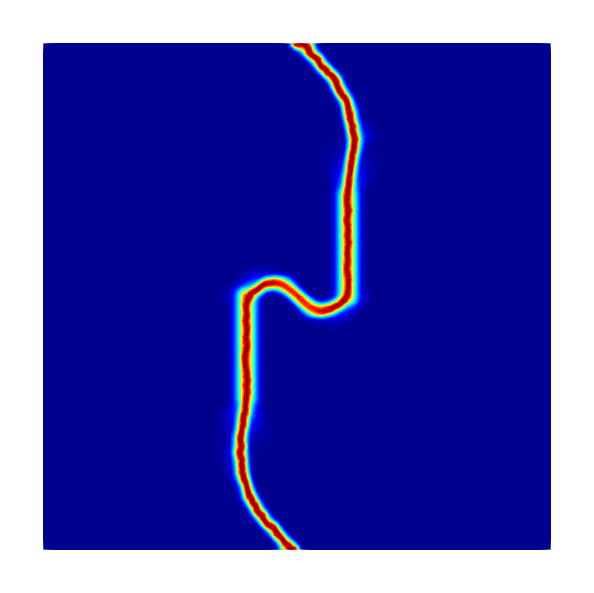
\includegraphics[width=\textwidth,scale=0.5]{Chapter4/figures/biaxial_nosplit_1.png}
    \caption{$\mathcal{D}^* = 0.14$}
    \label{fig: Chapter4/biaxial_nosplit_1}
  \end{subfigure}
  \hspace{0.03\textwidth}
  \begin{subfigure}[b]{0.23\textwidth}
    \centering
    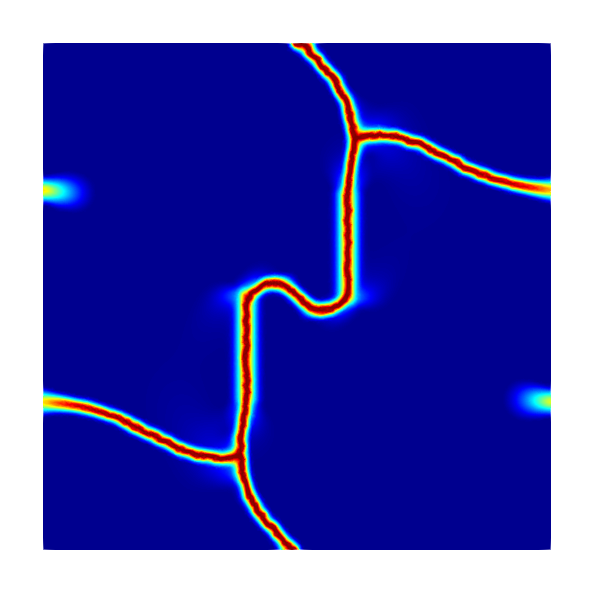
\includegraphics[width=\textwidth,scale=0.5]{Chapter4/figures/biaxial_nosplit_2.png}
    \caption{$\mathcal{D}^* = 0.19$}
    \label{fig: Chapter4/biaxial_nosplit_2}
  \end{subfigure}
  \hspace{0.03\textwidth}
  \begin{subfigure}[b]{0.23\textwidth}
    \centering
    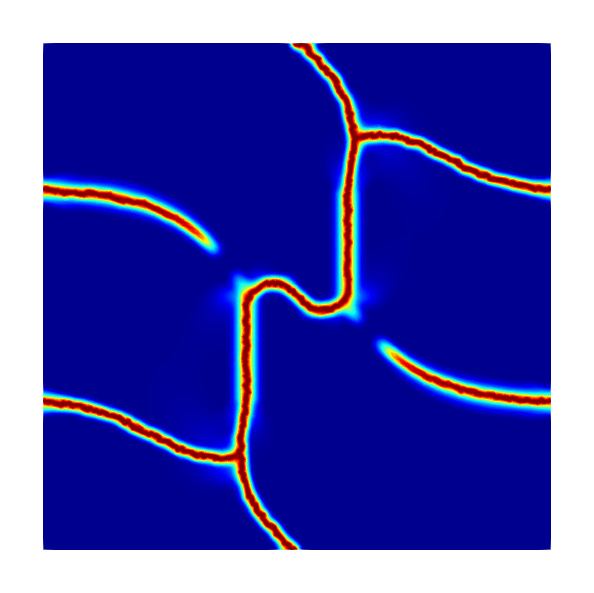
\includegraphics[width=\textwidth,scale=0.5]{Chapter4/figures/biaxial_nosplit_3.png}
    \caption{$\mathcal{D}^* = 0.75$}
    \label{fig: Chapter4/biaxial_nosplit_3}
  \end{subfigure}
  \begin{subfigure}[b]{0.065\textwidth}
    \centering
    \caption*{d}
    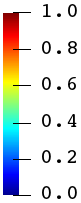
\includegraphics[width=\textwidth]{Chapter4/figures/jet_vertical.png}
    \vspace{0.15in}
  \end{subfigure}
  
  \begin{subfigure}[b]{0.23\textwidth}
    \centering
    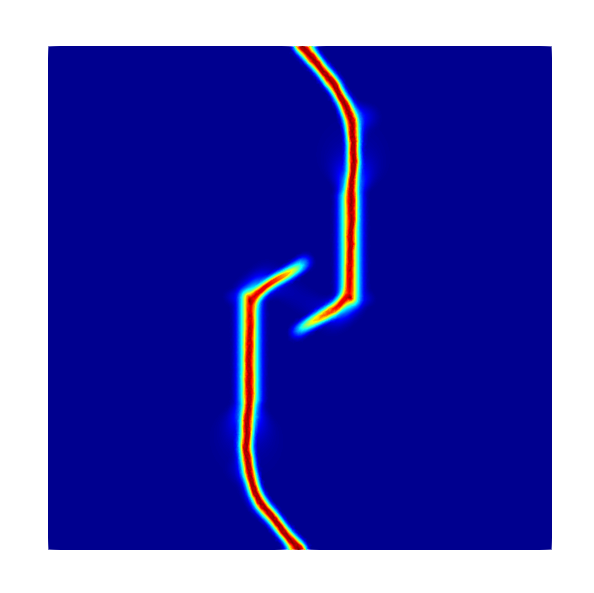
\includegraphics[width=\textwidth,scale=0.5]{Chapter4/figures/biaxial_spectral_1.png}
    \caption{$\mathcal{D}^* = 0.14$}
    \label{fig: Chapter4/biaxial_spectral_1}
  \end{subfigure}
  \hspace{0.03\textwidth}
  \begin{subfigure}[b]{0.23\textwidth}
    \centering
    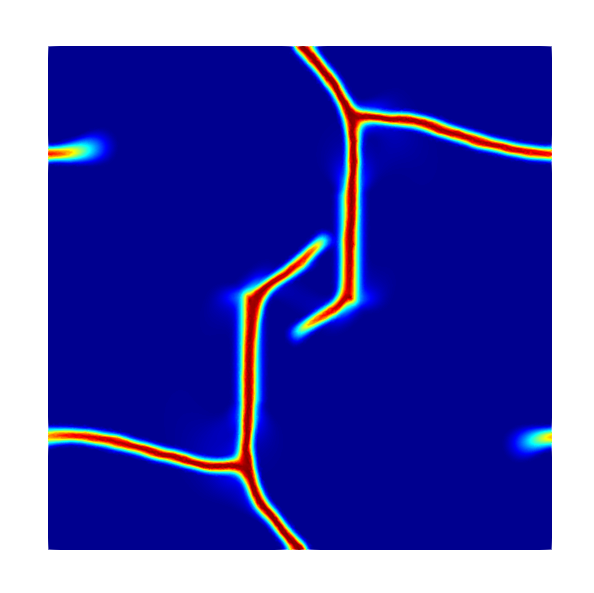
\includegraphics[width=\textwidth,scale=0.5]{Chapter4/figures/biaxial_spectral_2.png}
    \caption{$\mathcal{D}^* = 0.19$}
    \label{fig: Chapter4/biaxial_spectral_2}
  \end{subfigure}
  \hspace{0.03\textwidth}
  \begin{subfigure}[b]{0.23\textwidth}
    \centering
    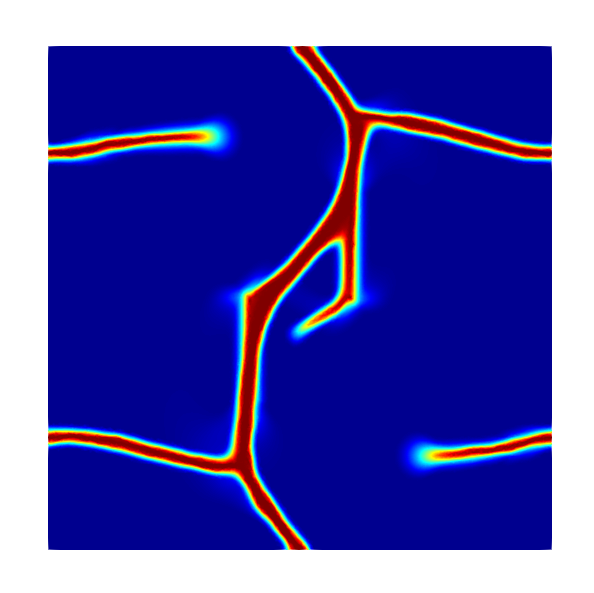
\includegraphics[width=\textwidth,scale=0.5]{Chapter4/figures/biaxial_spectral_3.png}
    \caption{$\mathcal{D}^* = 0.75$}
    \label{fig: Chapter4/biaxial_spectral_3}
  \end{subfigure}
  \begin{subfigure}[b]{0.065\textwidth}
    \centering
    \caption*{d}
    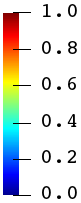
\includegraphics[width=\textwidth]{Chapter4/figures/jet_vertical.png}
    \vspace{0.15in}
  \end{subfigure}
  
  \begin{subfigure}[b]{0.23\textwidth}
    \centering
    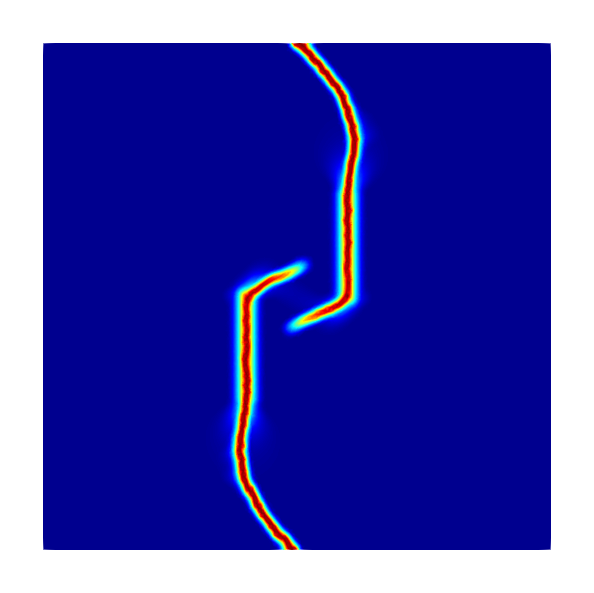
\includegraphics[width=\textwidth,scale=0.5]{Chapter4/figures/biaxial_odd_1.png}
    \caption{$\mathcal{D}^* = 0.14$}
    \label{fig: Chapter4/biaxial_odd_1}
  \end{subfigure}
  \hspace{0.03\textwidth}
  \begin{subfigure}[b]{0.23\textwidth}
    \centering
    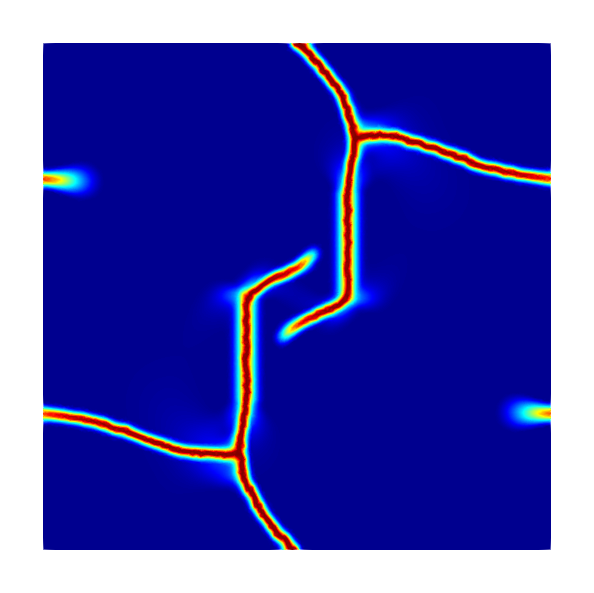
\includegraphics[width=\textwidth,scale=0.5]{Chapter4/figures/biaxial_odd_2.png}
    \caption{$\mathcal{D}^* = 0.19$}
    \label{fig: Chapter4/biaxial_odd_2}
  \end{subfigure}
  \hspace{0.03\textwidth}
  \begin{subfigure}[b]{0.23\textwidth}
    \centering
    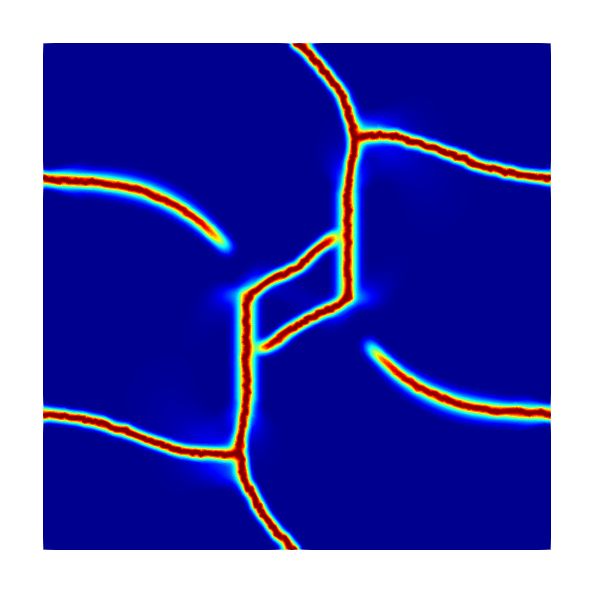
\includegraphics[width=\textwidth,scale=0.5]{Chapter4/figures/biaxial_odd_3.png}
    \caption{$\mathcal{D}^* = 0.75$}
    \label{fig: Chapter4/biaxial_odd_3}
  \end{subfigure}
  \begin{subfigure}[b]{0.065\textwidth}
    \centering
    \caption*{d}
    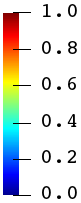
\includegraphics[width=\textwidth]{Chapter4/figures/jet_vertical.png}
    \vspace{0.15in}
  \end{subfigure}
  \caption[The crack paths for the biaxial tension test.]{The crack paths obtained using (a-c) a no-split technique (d-f) the spectral decomposition (g-i) the contact split. }
  \label{fig: Chapter4/biaxial_crack_path}
\end{figure}
